%%%%%%%%%%%%%%%%%%%%%%%%%%%%%%%%%%%%%%%%%
% a0poster Portrait Poster
% LaTeX Template
% Version 1.0 (22/06/13)
%
% The a0poster class was created by:
% Gerlinde Kettl and Matthias Weiser (tex@kettl.de)
%
% This template has been downloaded from:
% http://www.LaTeXTemplates.com
%
% License:
% CC BY-NC-SA 3.0 (http://creativecommons.org/licenses/by-nc-sa/3.0/)
%
%%%%%%%%%%%%%%%%%%%%%%%%%%%%%%%%%%%%%%%%%

%----------------------------------------------------------------------------------------
%	PACKAGES AND OTHER DOCUMENT CONFIGURATIONS
%----------------------------------------------------------------------------------------

\documentclass[a0,portrait]{a0poster}

\usepackage{multicol} % This is so we can have multiple columns of text side-by-side
\columnsep=100pt % This is the amount of white space between the columns in the poster
\columnseprule=3pt % This is the thickness of the black line between the columns in the poster

\usepackage[svgnames]{xcolor} % Specify colors by their 'svgnames', for a full list of all colors available see here: http://www.latextemplates.com/svgnames-colors

%\usepackage{times} % Use the times font
\usepackage{palatino} % Uncomment to use the Palatino font

\usepackage{graphicx} % Required for including images
\graphicspath{{figures/}} % Location of the graphics files
\usepackage{booktabs} % Top and bottom rules for table
\usepackage[font=small,labelfont=bf]{caption} % Required for specifying captions to tables and figures
\usepackage{amsfonts, amsmath, amsthm, amssymb} % For math fonts, symbols and environments
\usepackage{wrapfig} % Allows wrapping text around tables and figures

\begin{document}

%----------------------------------------------------------------------------------------
%	POSTER HEADER
%----------------------------------------------------------------------------------------

% The header is divided into two boxes:
% The first is 75% wide and houses the title, subtitle, names, university/organization and contact information
% The second is 25% wide and houses a logo for your university/organization or a photo of you
% The widths of these boxes can be easily edited to accommodate your content as you see fit
\begin{minipage}[b]{0.75\linewidth}
  \veryHuge \color{NavyBlue} \textbf{\textsc{Does structure in neural \\[0.3cm] activity match anatomical structure?}} \color{Black}\\[1cm] % Title
  % \Huge\textit{An Exploration of Complexity}\\[2cm] % Subtitle
  \huge \textbf{Thomas Delaney, Dr. Cian O'Donnell}\\[0.3cm] % Author(s)
  \huge University of Bristol, Dept of Computer Science\\[0.1cm] % University/organization
  \large \texttt{bristolcnu.github.io} \\
  \Large \texttt{t.delaney@bristol.ac.uk} \\
\end{minipage}
%
\begin{minipage}[b]{0.24\linewidth}
  \centering
  
\includegraphics[width=0.9\linewidth]{bristol_university_logo.png} \vspace{0.3cm}\\
  
\includegraphics[width=0.9\linewidth]{epsrc_logo.png} \vspace{2.7cm}\\
\end{minipage}
%\vspace{0.5cm} % A bit of extra whitespace between the header and poster content

%----------------------------------------------------------------------------------------

\begin{multicols}{2} % This is how many columns your poster will be broken into, a portrait poster is generally split into 2 columns

%----------------------------------------------------------------------------------------
%	ABSTRACT
%----------------------------------------------------------------------------------------
%
% \color{Navy} % Navy color for the abstract
%
% \begin{abstract}
%
% Sed fringilla tempus hendrerit. Vestibulum ante ipsum primis in faucibus orci luctus et ultrices posuere cubilia Curae; Etiam ut elit sit amet metus lobortis consequat sit amet in libero. Lorem ipsum dolor sit amet, consectetur adipiscing elit. Phasellus vel sem magna. Nunc at convallis urna. isus ante. Pellentesque condimentum dui. Etiam sagittis purus non tellus tempor volutpat. Donec et dui non massa tristique adipiscing. Quisque vestibulum eros eu. Phasellus imperdiet, tortor vitae congue bibendum, felis enim sagittis lorem, et volutpat ante orci sagittis mi. Morbi rutrum laoreet semper. Morbi accumsan enim nec tortor consectetur non commodo nisi sollicitudin. Proin sollicitudin. Pellentesque eget orci eros. Fusce ultricies, tellus et pellentesque fringilla, ante massa luctus libero, quis tristique purus urna nec nibh.
%
% \end{abstract}

%----------------------------------------------------------------------------------------
%	INTRODUCTION
%----------------------------------------------------------------------------------------

%\color{SaddleBrown} % SaddleBrown color for the introduction

\section*{\color{NavyBlue}\textsc{Introduction}\color{Black}}

Information in the brain is carried in correlated network activity. Until recently, it has been difficult to record responses from multiple brain regions simultaneously. This meant that studies on network behaviour were restricted to studying only one region at a time. The development of `Neuropixels' probes have allowed extracellular voltage measurements to be collected from multiple brain regions simultaneously. In this project, we used data collected from five different brain regions to compare distributions of correlated activity within these regions, and between these regions.

We then used these measurements to create networks between the neurons in these five regions. We used a cutting edge community detection algorithm to find communities in these networks. We are currently in the process of comparing these communities to the anatomical distribution of their constituents.

%----------------------------------------------------------------------------------------
%	OBJECTIVES
%----------------------------------------------------------------------------------------

% \color{DarkSlateGray} % DarkSlateGray color for the rest of the content

\section*{\color{NavyBlue}\textsc{Main Objectives}\color{NavyBlue}}

\begin{enumerate}
  \item To compare the distributions of spike count correlations ($r_{SC}$) and mutual information ($I(X;Y)$) in different regions.
  \item To examine the relationship between these measurements and firing rates across all regions.
  \item To detect any communities in the networks created by these measurements, either within or between the anatomical regions.
  \item To compare the network communities to their anatomical distribution.
\end{enumerate}

%----------------------------------------------------------------------------------------
%	DATA
%----------------------------------------------------------------------------------------

\section*{\color{NavyBlue}\textsc{Data}\color{NavyBlue}}

Using two probes, spiking activity was simultaneously collected from over 800 neurons in an awake mouse brain for a period of 84 minutes. During this period, the mouse and was shown various visual stimuli. The 800 neurons were distributed across 5 different brain regions: \textbf{V1, hippocampus, thalamus, motor cortex}, and \textbf{striatum} \cite{jun}.

\begin{minipage}[b]{0.9\linewidth}
  \begin{center}
  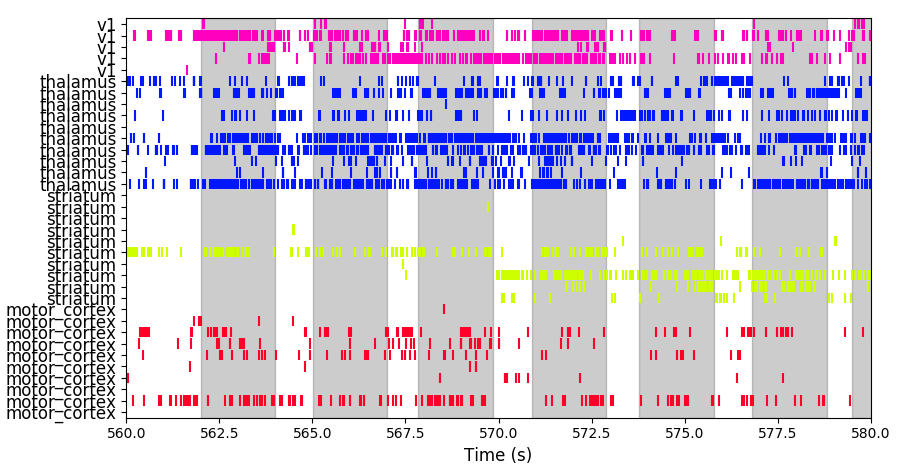
\includegraphics[width=0.9\linewidth, height=13cm]{raster_plot.png}
  \end{center}
\end{minipage}
%
\begin{minipage}[b]{0.1\linewidth}
  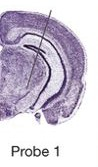
\includegraphics[width=\linewidth, height=5cm]{probe_1.jpg} \\
  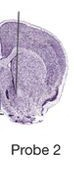
\includegraphics[width=0.9\linewidth, height=6.5cm]{probe_2.jpg} % \vspace{2.5cm}
\end{minipage}

\captionof{figure}{(Left) A raster plot showing the firing times of a subset of the cells, during a subset of the experiment time. Shaded areas indicate times when a visual stimulus was present, and (Right) Positions of the two probes. Probe 1 intersects V1, the hippocampus, and the thalamus. Probe 2 intersects the motor cortex and the striatum.}

%----------------------------------------------------------------------------------------
%	MATERIALS AND METHODS
%----------------------------------------------------------------------------------------

\section*{\color{NavyBlue}\textsc{Materials and Methods}\color{Black}}

\begin{description}
  \item[Spike Count Correlation, $r_{SC}$] We measured Pearson's correlation between the spike counts of neurons in pairs.
  \item[Mutual Information, $I(X;Y)$] We measured the mutual information between the spike counts of neurons in pairs.
  \item[Network Noise Rejection] We used a recently developed method to split the networks created by these measures into signal and noise networks \cite{humphries}.
  \item[Consensus Clustering] We used consensus clustering on the signal network to investigate any communities within these networks \cite{humphries}.
\end{description}

%----------------------------------------------------------------------------------------
%	RESULTS
%----------------------------------------------------------------------------------------

\section*{\color{NavyBlue}\textsc{Results}\color{Black}}

\subsection*{\color{NavyBlue}\textsc{Correlation \& Information Distributions}\color{Black}}

We used a statistical test to find out if the distributions of pairwise correlations were different between regions. We found that correlations in the hippocampus and thalamus were statistically different to those in the other three regions ($p < 0.05$).

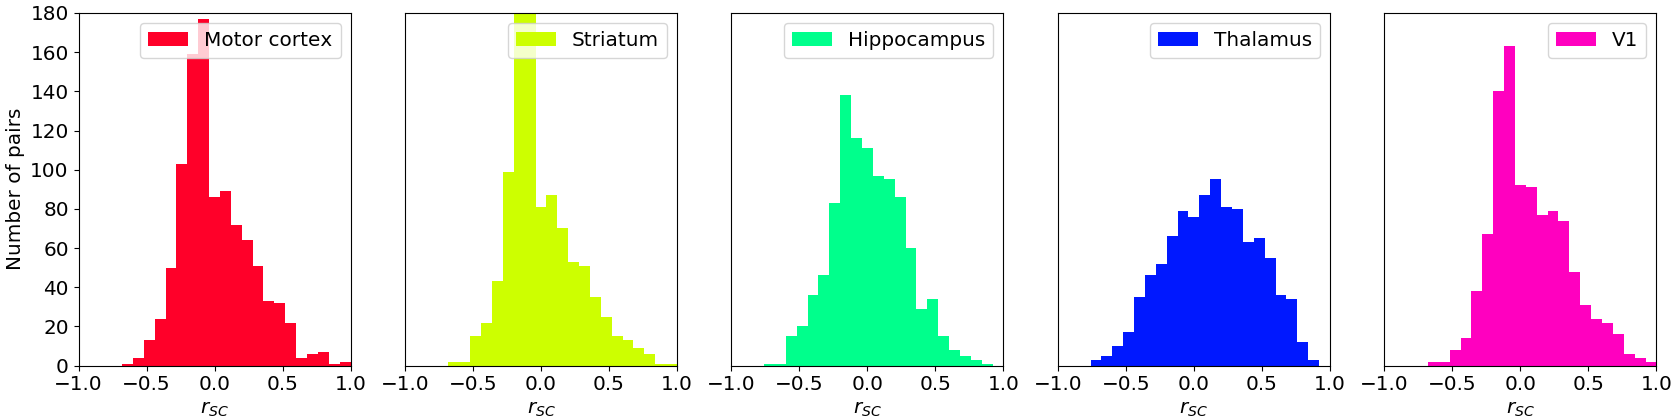
\includegraphics[width=\linewidth, height=7.5cm]{correlation_histograms.png}
\captionof{figure}{Histograms of the spike count correlations of 1000 randomly chosen pairs of neurons from within each region.}

We did the same for mutual information distributions. Comparing all pairwise combinations of regions, we found that all regional distributions of mutual information were statistically different ($p < 0.001$).

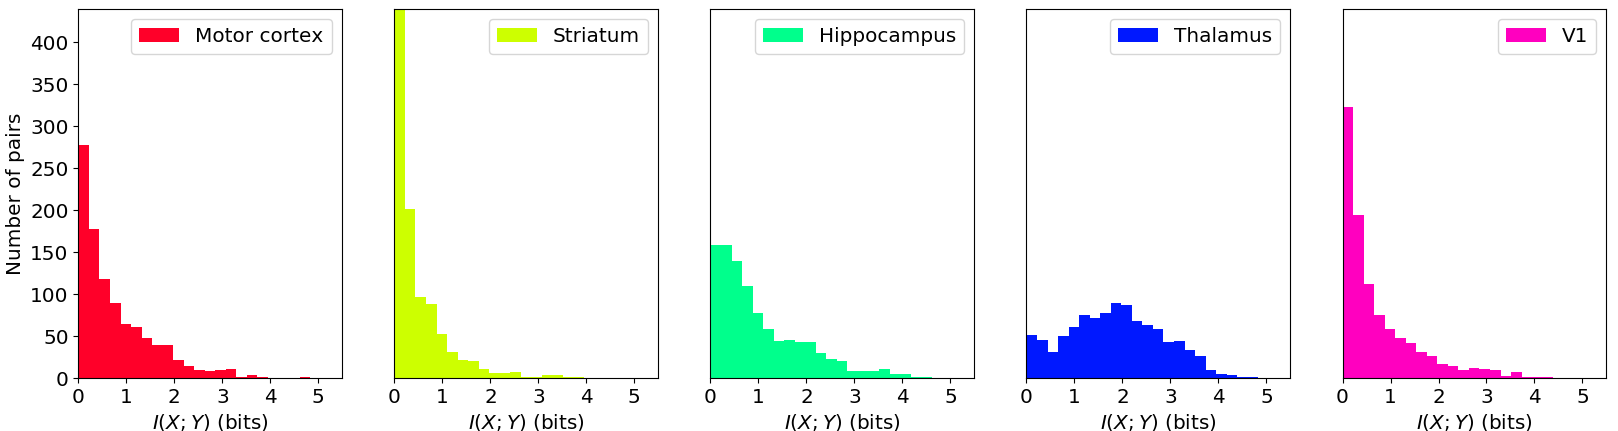
\includegraphics[width=\linewidth, height=7.5cm]{information_histograms.png}
\captionof{figure}{Histograms of the mutual information between the spike counts of 1000 randomly chosen pairs of neurons from within each region.}

\subsection*{\color{NavyBlue}\textsc{Pairwise Geomtric Mean, Correlation \& Information}\color{Black}}

We compared the spike count correlations for pairs of neurons to the geometric means of their firing rates. Surprisingly, we found very little correlation between the two quantities.

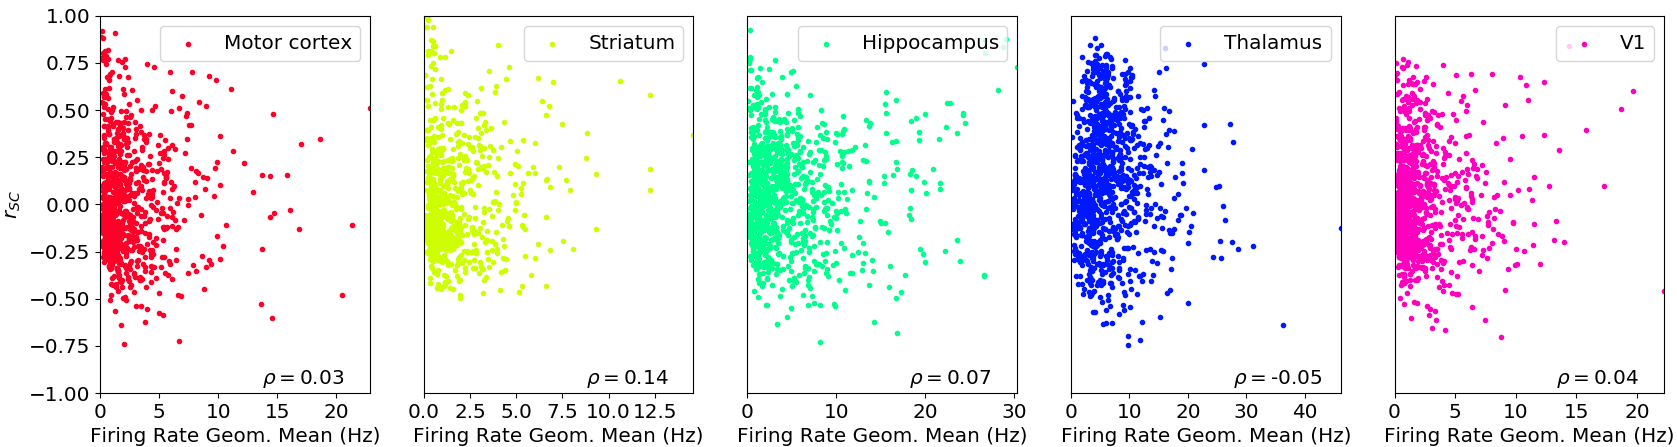
\includegraphics[width=\linewidth, height=7.5cm]{correlation_vs_geometric_mean.png}
\captionof{figure}{Spike count correlations of pairs of neurons plotted against geometric means of the firing rate of those pairs for each region.}

We found a strong positive correlation between the pairwise geometric mean and the mutual information.

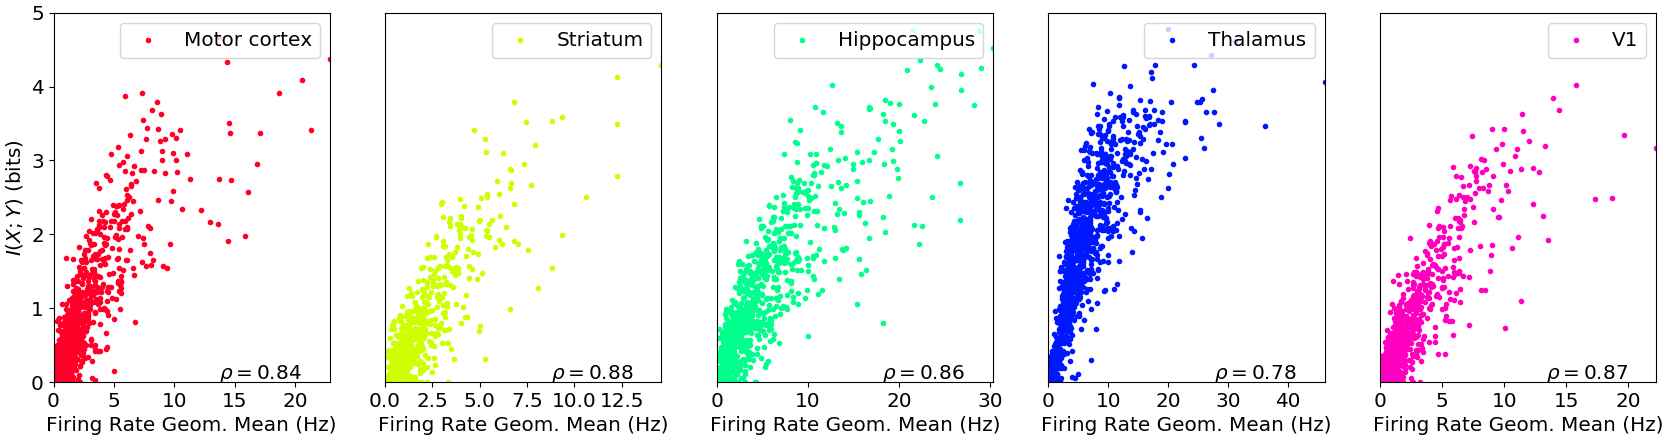
\includegraphics[width=\linewidth, height=7.5cm]{info_vs_geometric_mean.png}
\captionof{figure}{Mutual information of pairs of neurons plotted against geometric means of the firing rate of those pairs for each region.}

We expected strong spike count correlations to correspond to relatively large values for the mutual information. So we scattered one quantity against the other and fitted a quadratic curve to the data. Whatever correlation we found between the two quantities was not as strong as we expected.

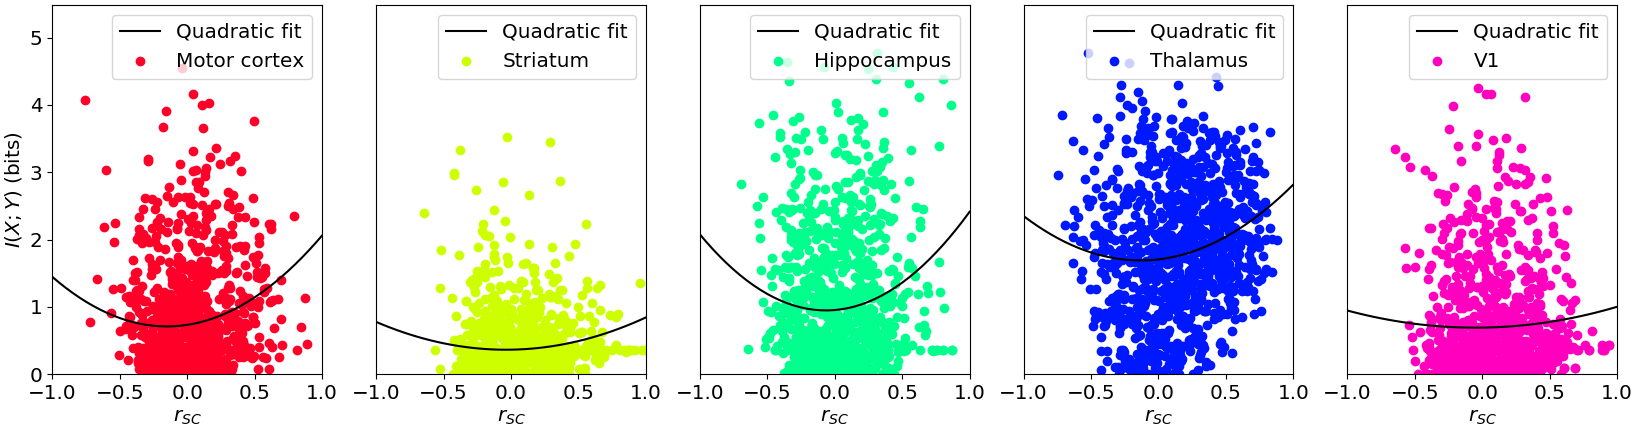
\includegraphics[width=\linewidth, height=7.5cm]{info_vs_corr.png}
\captionof{figure}{Mutual information of pairs of neurons plotted against the spike count correlations of those pairs for each region.}

\subsection*{\color{NavyBlue}\textsc{Community Detection}\color{Black}}

Using Network Noise Rejection and Consensus Clustering, we detected two communities in the network created by the mutual information measurements. It appears that one community is dominated by the thalamus, and the other community is dominated by the motor cortex and striatum.

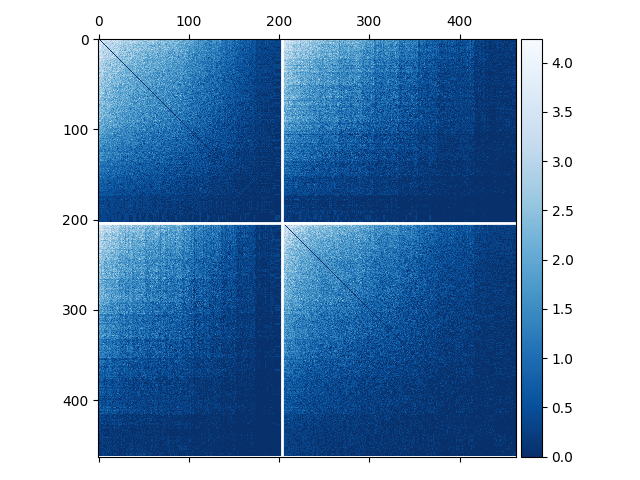
\includegraphics[width=0.5\linewidth]{cons_cluster_map_all_good_15.png}
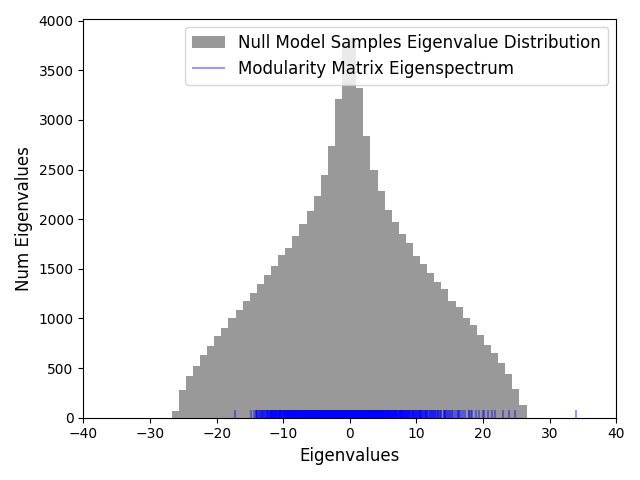
\includegraphics[width=0.5\linewidth]{eig_hist_all_good_15.png}
\captionof{figure}{(Left) Mutual information matrix of the signal network, with communities shown. Main diagonal entries set to zero. (Right) A histogram of the eigenvalues of the samples from the null model, with the eigenvalues of the modularity matrix of the network shown in blue.}


%----------------------------------------------------------------------------------------
%	CONCLUSIONS
%----------------------------------------------------------------------------------------

\section*{\color{NavyBlue}\textsc{Conclusions}\color{Black}}

\begin{itemize}
  \item The pairwise measurements we took were distributed differently in different brain regions.
  \item The mutual information between two cells is strongly correlated with the geometric mean of their firing rates.
  \item Functional communities exist across anatomical regions.
  \item The thalamus appears to be more isolated functionally than the other anatomical regions.
\end{itemize}

%----------------------------------------------------------------------------------------
%	FORTHCOMING RESEARCH
%----------------------------------------------------------------------------------------

\section*{\color{NavyBlue}\textsc{Forthcoming Research}\color{Black}}

Different pairwise measurements could be used along with the community detection. Alternatively, higher order correlation measures, such as population coupling could be examined. Changes in community structure in response to different stimuli could be examined.

%----------------------------------------------------------------------------------------
%	ACKNOWLEDGEMENTS
%----------------------------------------------------------------------------------------

\section*{\color{NavyBlue}\textsc{Acknowledgements}\color{Black}}

I would like to thank Dr. Nick Steinmetz (University of Washington, Seattle) for making the dataset used in this project publicly available.

 %----------------------------------------------------------------------------------------
%	REFERENCES
%----------------------------------------------------------------------------------------

% \nocite{*} % Print all references regardless of whether they were cited in the poster or not
\bibliography{conference_poster_6.bbl} % Use the example bibliography file sample.bib

%----------------------------------------------------------------------------------------

\end{multicols}
\end{document}
